\documentclass{article}

% if you need to pass options to natbib, use, e.g.:
% \PassOptionsToPackage{numbers, compress}{natbib}
% before loading nips_2018

% ready for submission
\usepackage{nips_2018}

% to compile a preprint version, e.g., for submission to arXiv, add
% add the [preprint] option:
% \usepackage[preprint]{nips_2018}

% to compile a camera-ready version, add the [final] option, e.g.:
% \usepackage[final]{nips_2018}

% to avoid loading the natbib package, add option nonatbib:
% \usepackage[nonatbib]{nips_2018}

\usepackage[utf8]{inputenc} % allow utf-8 input
\usepackage[T1]{fontenc}    % use 8-bit T1 fonts
\usepackage{hyperref}       % hyperlinks
\usepackage{url}            % simple URL typesetting
\usepackage{booktabs}       % professional-quality tables
\usepackage{amsfonts}       % blackboard math symbols
\usepackage{nicefrac}       % compact symbols for 1/2, etc.
\usepackage{microtype}      % microtypography


% Added by Wenlong Lyu
\usepackage{amsmath}
\usepackage[plain]{fancyref}
\usepackage{bm}
\usepackage{todonotes}
\usepackage{placeins}
\usepackage{multirow}
\usepackage{longtable}

\title{Multi-task Neural Network for Multi-output Gaussian Process Regression}

% The \author macro works with any number of authors. There are two
% commands used to separate the names and addresses of multiple
% authors: \And and \AND.
%
% Using \And between authors leaves it to LaTeX to determine where to
% break the lines. Using \AND forces a line break at that point. So,
% if LaTeX puts 3 of 4 authors names on the first line, and the last
% on the second line, try using \AND instead of \And before the third
% author name.

\author{
  Wenlong Lyu \\
  School of Microelectronics, Fudan University\\
  \texttt{wllv16@fudan.edu.cn} \\
  %% examples of more authors
  %% \And
  %% Coauthor \\
  %% Affiliation \\
  %% Address \\
  %% \texttt{email} \\
  %% \AND
  %% Coauthor \\
  %% Affiliation \\
  %% Address \\
  %% \texttt{email} \\
  %% \And
  %% Coauthor \\
  %% Affiliation \\
  %% Address \\
  %% \texttt{email} \\
  %% \And
  %% Coauthor \\
  %% Affiliation \\
  %% Address \\
  %% \texttt{email} \\
}

\begin{document}
% \nipsfinalcopy is no longer used

\maketitle


\begin{abstract}
The last hidden layer of a neural network can be viewed as a finite feature map, from which a reduced-rank Gaussian process model can be built. On the other hand, multiple correlated outputs can be represented by a neural network with shared hidden layers. In this paper, we propose a simple multi-output Gaussian process regression model based the two ideas. The kernel functions of multiple outputs are constructed from a multi-task neural network with shared hidden layers and task-specific layers. The correlations are captured by the shared hidden layers. We compare our multi-task neural network enhanced Gaussian process (MTNN-GP) model with several multi-output Gaussian process models using two public datasets and one example of real-world analog integrated circuits, the results show that our model is competitive compared with these models.
\end{abstract}

\section{Introduction}

% Gaussian process regression is important, as it models the uncertainty, so the it \emph{know what it knows}.
The Gaussian process (GP) regression is popular as the model provides the predictions as well as the well-calibrated uncertainties. The uncertainty estimation makes the model more robust to unseen events as the model \emph{knows what it knows}. The conventional GP models are usually designed to learn a scalar-valued function. However, in some scenarios, we need to model a vector-valued function, and the multiple outputs are possibly correlated. Instead of treating the vector-valued function as multiple separate scalar-valued functions, the multi-output learning \cite{zhang2017survey} tries to build a unified model and simultaneously learn all the outputs. The overall performance could be enhanced by exploiting the correlations of the tasks.

% Existing methods: convolution based, krok based, GPRN.
Multi-task Gaussian process \cite{vectorvaluedkernel} tries to combine multi-task learning and Gaussian process. The linear model of coregionalization (LMC) methods \cite{journel1978mining} assume the $Q$ outputs $f_i(\bm{x}), i \in \{1\dots Q\}$ are linear combinations of several latent functions as $f_i(\bm{x}) = \sum_{j=1}^U a_{ij} u_j(\bm{x})$. In \cite{bonilla2008multi}, the covariance matrix is expressed as the Kronecker product of the task covariance and the task-irrelevant input covariance matrix. In \cite{nguyen2014collaborative}, the output function $f_i(\bm{x})$ is expressed as the linear combinations of $U$ latent functions $u_j(\bm{x}), j \in \{1\dots U\}$ plus a task-specific function $h_i(\bm{x})$, efficient training and inference methods are also developed. In the Gaussian process regression network (GPRN) model~\cite{wilson2012gaussian}, the $i$-th output function $f_i(\bm{x})$ is also expressed as weighted combinations of $U$ latent functions. However, the weights are also nonlinear functions characterized by GP so that $f_i(\bm{x}) = \sum_{j=1}^U w_{ij}(\bm{x}) (u_j(\bm{x}) + \epsilon_u) + \epsilon_f$ where $\epsilon_u$ and $\epsilon_f$ are the noise terms. Another methodology of building multi-task kernels is \emph{process convolution} \cite{boyle2005dependent,alvarez2009sparse,alvarez2011computationally}, where the output function $f_i(\bm{x})$ is assumed to be the convolution of output-dependent smoothing kernel $g_i(\bm{x})$ and a latent function $u(\bm{x})$.

In this paper, we propose a multi-output Gaussian process model based on the multi-task neural network. As a degenerate GP can be built from a finite feature map and neural networks can generate representative features, a degenerate GP can be derived from a neural with finite hidden units \cite{lazaro2010marginalized, huang2015scalable}. In our proposed model, the multi-output GP is built from a deep neural network with shared layers and task-specific layers. The input data is first transformed into \emph{shared features} through the shared layers and further mapped to \emph{task-specific features} by each task's task-specific layers. GP kernels for the outputs are then built from the inner product of the task-specific features. The weights of the multi-task neural network is obtained by maximizing the likelihood with gradient back-propagation.

We compared our model with independent GP model and several multi-output GP models using three datasets, including two public datasets and one dataset from the simulation results of a real-world analog integrated circuit. We demonstrate that our model can provide better predictions and uncertainty estimations than the compared models.

The rest of the paper is organized as follows. In \Fref{sec:Background}, we present the background of the Gaussian process and GP model built from neural networks with finite hidden units. In \Fref{sec:mogp}, we present our proposed multi-output GP model via multi-task neural network. The experimental results are given in \Fref{sec:experiments}. We conclude the paper in \Fref{sec:conclusion}.
% XXX:
% advantage:
%   the correlation modeling is more flexibility
%   efficient

% XXX:
% Kronecker product: the covaiance matrix is decomposed as the Kronecker product of covaiance of task and covaiance of input
% GPRN: $\bm{f}(x) = W(\bm{x})^T \bm{lf}(\bm{x})$, where $\bm{x}$ and $W(\bm{x})$ are GP
% convolution:

\section{Background}\label{sec:Background}

\subsection{Gaussian Process Regression}\label{sec:SOGP}

Given a training set $D_T = \{X, \bm{y}\}$ where $X = \{\bm{x}_1,~\dots~\bm{x}_N\}$, and $\bm{y} = \{y_1,~\dots~y_N\}$, we assume the target value $y$ is generated
by a latent function $f(\bm{x})$ with additive noise $\epsilon \sim N(0, \sigma_n^2)$ such that
\begin{equation}
    \label{eq:yf}
    y_i \sim N(f(\bm{x}_i), \sigma_n^2)
    % y_i = f(\bm{x}_i) + \epsilon_i.
\end{equation}
Here $N(\cdot, \cdot)$ denotes a Gaussian distribution. We use Gaussian process (GP)~\cite{GPML} to learn the latent function $f(\bm{x})$. A GP model defines a prior over $f(\bm{x})$. GP is fully characterized by a mean function $m(\bm{x})$ and a covariance function $k(\bm{x}, \bm{y})$. For the training set $D_T$, the latent function values $\bm{f} = (f(\bm{x}_1),~\dots~f(\bm{x}_N))^T$ follow a joint Gaussian distribution $\bm{f} \sim N(\bm{m}, K)$, where $\bm{m} = (m(\bm{x}_1),~\dots~,m(\bm{x}_N))^T$ is the mean vector, and $K_{ij} = k(\bm{x}_i, \bm{x}_j)$ is the covariance matrix. The mean function $m(\bm{x})$ can be any function, while the kernel function $k(\bm{x}, \bm{y})$ has to make sure that the covariance matrix is a symmetric positive definite (SPD) matrix. In this paper, we fix $m(\bm{x}) = 0$.

Given a new input $\bm{x}_*$, GP model predicts the distribution of the output, i.e., $y \sim N(\mu(\bm{x}_*), \sigma^2(\bm{x}_*))$, where $\mu(\bm{x}_*)$ and $\sigma^2(\bm{x}_*)$ can be expressed as

\begin{equation}
    \left\{
        \begin{array}{lll}
            \mu(\bm{x}_*)      &=& k(\bm{x}_*, X) (K + \sigma_n^2 I)^{-1} \bm{y} \\
            \sigma^2(\bm{x}_*) &=& \sigma_n^2 + k(\bm{x}_*, \bm{x}_*) - k(\bm{x}_*, X) (K + \sigma_n^2 I)^{-1} k(X, \bm{x}_*),
        \end{array}
    \right.
    \label{eq:GPRPred}
\end{equation}

where $k(\bm{x}_*, X) = (k(\bm{x}_*, \bm{x}_1),~\dots~,k(\bm{x}_*, \bm{x}_N))$ and $k(X, \bm{x}_*) = k(\bm{x}_*, X)^T$. In \eqref{eq:GPRPred}, $\mu(\bm{x}_*)$ and $\sigma^2(\bm{x}_*)$ and be viewed as the prediction and the uncertainty measure.

There are usually some hyperparameters for a GP model, including the noise level $\sigma_n$ and the hyperparameters for the kernel functions. For example, the squared exponential kernel is a commonly used kernel in GP regression. The kernel function is defined as

\begin{equation}
    \label{eq:GaussianCovarianceFunction}
    k(\bm{x}_i, \bm{x}_j) = \sigma_f^2 \exp\Big(-\frac{1}{2}(\bm{x}_i - \bm{x}_j)^T\Lambda^{-1}(\bm{x}_i - \bm{x}_j)\Big),
\end{equation}
where $\Lambda = \mathrm{diag}(l_1, \dots, l_d)$ is a diagonal matrix and $l_i$ denotes the length scale of the $i$-th dimension. $\sigma_f$ and $\Lambda$ are the hyperparameters for the kernel. Denote $\bm{\theta}$ as the vector of hyperparameters, the hyperparameters can be learned via maximum likelihood estimation (MLE) by maximizing the following likelihood function

\begin{equation}
    \label{eq:GPloglikelihood}
    \log p(\bm{y} | X, \bm{\theta}) = -\frac{1}{2}(\bm{y}^T K_{\bm{\theta}}^{-1} \bm{y} + \log |K_{\theta}| + N \log(2 \pi))
\end{equation}

Where $K_{\bm{\theta}}$ is the covariance matrix of the training input calculated by the kernel function.

\subsection{Reduced-Rank Gaussian Process Model from Finite-Dimensional Feature Map}\label{sec:NNGP}

\begin{figure}[!htb]
    \centering
    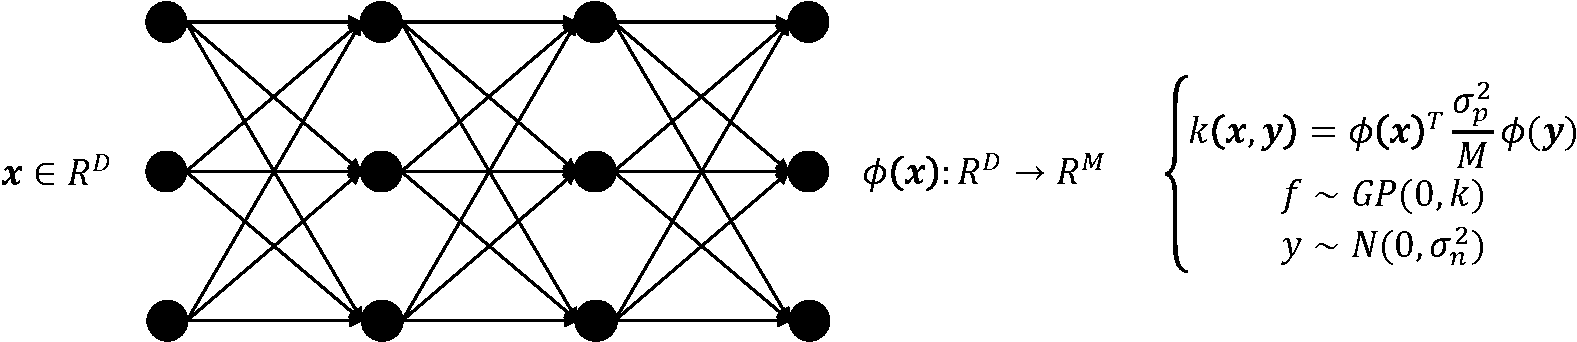
\includegraphics[width=\columnwidth]{./img/nn1.pdf}
    \caption{Architecture of the Gaussian process model with kernel characterized by deep neural network}
    \label{fig:NNGP}
\end{figure}

A Gaussian process model can also be derived from a weight space view. Let $\phi(\bm{x}): R^D \rightarrow R^M$ be a feature map from $D$-dimensional input space to the $M$-dimensional feature space. We assume that the latent function $f(\bm{x})$ is a linear combination of the nonlinear features, and the observed target values are generated from $f(\bm{x})$ with additive noise

\begin{equation}
    \label{eq:weightspace}
    \begin{array}{lll}
        f(\bm{x}) &=&    \bm{w}^T \phi(\bm{x})   \\
        y_i       &=&    f(\bm{x_i}) + \epsilon  \\
        \epsilon  &\sim& N(0, \sigma_n^2)
    \end{array}.
\end{equation}

If a zeros mean Gaussian prior with covariance matrix $\Sigma_p$ is imposed on the weights $\bm{w}$, i.e., $\bm{w} \sim N(0, \Sigma_p)$, it can be proved that $f$ follows a Gaussian process $f \sim \mathcal{GP}(0, k)$ \cite{GPML}, with the kernel function $k$ defined as
\begin{equation}
    \label{eq:kernel_from_weight}
    k(\bm{x}, \bm{y}) = \phi(\bm{x})^T \Sigma_p \phi(\bm{y}).
\end{equation}
The GP model defined from finite feature map is called \emph{degenerate} Gaussian process, as the covariance matrix calculated from \eqref{eq:kernel_from_weight} would have a lower rank $M$ than $N$.

%XXX: mension the matrix inversion lemma

If we set $\Sigma_p$ to a diagonal matrix $\Sigma_p = \frac{\sigma_p^2}{M} I$\cite{lazaro2010marginalized}, the predictive distribution of \eqref{eq:GPRPred} can be reformulated as
\begin{equation}
    \left\{
        \begin{array}{lll}
            \mu(\bm{x})      &= & \phi(x)^T A^{-1} \Phi \bm{y} \\
            \sigma^2(\bm{x}) &= & \sigma_n^2 + \sigma_n^2 \phi(\bm{x})^T A^{-1} \phi(\bm{x}) \\
            \Phi             &= & (\phi(\bm{x}_1),~\dots~,\phi(\bm{x}_N)) \\
            A                &= & \Phi \Phi^T + \frac{M \sigma_n^2}{\sigma_p^2} I
        \end{array}.
    \right.
    \label{eq:DegeneratePred}
\end{equation}

Note that the when calculating $\mu(\bm{x})$ and $\sigma^2(\bm{x})$ directly using \eqref{eq:GPRPred}, the time complexity are $O(N)$ and $O(N^2)$, respectively. However, if \eqref{eq:DegeneratePred} is used, the time complexity for calculating $\mu(\bm{x})$ and $\sigma^2(\bm{x})$ become $O(M)$ and $O(M^2)$ as long as the inverse of $A$ is pre-calculated.

The log likelihood of the training data defined in \eqref{eq:GPloglikelihood} can also be reformulated as \cite{lazaro2010marginalized}
\begin{equation}
    \label{eq:DegenerateGPloglikelihood}
    \log p(\bm{y} | X, \bm{\theta}) = -\frac{1}{2\sigma_n^2}(\bm{y}^T\bm{y} - \bm{y}^T \Phi^T A^{-1} \Phi \bm{y}) - \frac{1}{2}\log |A| + \frac{M}{2} \log \frac{M \sigma_n^2}{\sigma_p^2} - \frac{N}{2} \log(2 \pi \sigma_n^2),
\end{equation}
where $\bm{\theta}$ is the vector containing $\sigma_p$, $\sigma_n$ and the parameters of $\phi$. In \eqref{eq:GPloglikelihood}, the covariance matrix $K$ should be inverted, which would take $O(N^3)$ operations. For \eqref{eq:DegenerateGPloglikelihood}, the matrix $A$ is of the size $M \times M$, so the time complexity for calculating \eqref{eq:DegenerateGPloglikelihood} is only $O(NM^2 + M^3)$.

% XXX: the loss function for the
It can be seen that GP model can be constructed from a finite feature map. Neural network (NN) can provide effective feature representations, it is thus natural to use a neural network as the feature map $\phi$. In \cite{lazaro2010marginalized}, a neural network with one hidden layer is proposed as the feature map $\phi(\bm{x})$. The weights of the neural network are obtained by maximizing the likelihood function in \eqref{eq:DegenerateGPloglikelihood} with gradient back-propagation. In \cite{huang2015scalable}, the single hidden layer is extended to multiple layers. The Gaussian process with kernel characterized by neural network is illustrated in \Fref{fig:NNGP}. A similar work is \cite{snoek2015scalable}, to perform Bayesian optimization, a neural network is firstly pre-trained, and Bayesian linear regression is then performed to the last layer.

% \paragraph{Deep ensemble}
\subsection{Model Averaging to Improve the Quality of Uncertainty Prediction}\label{sec:deepensemble}

When probabilistic models are built from neural networks, a simple model averaging technique\cite{lazaro2010marginalized, huang2015scalable, lakshminarayanan2017simple} can significantly improve the quality of the estimated uncertainty.

Firstly, $K$ independent probabilistic neural network models are trained with random initializations. Each model would give predictive distribution $p(y | \bm{x}, \bm{\theta}_k) = N(\mu_k(\bm{x}), \sigma_k^2(\bm{x}))$ where $\bm{\theta}_k$ is the neural network parameters for the $k$-th model, $\mu_k(\bm{x})$ and $\sigma_k^2(\bm{x})$ are the mean and variance of the corresponding predictive Gaussian distribution. The final predictive distribution can be expressed as $p(y | \bm{x}) = N(\mu(\bm{x}), \sigma^2(\bm{x}))$, where
\begin{equation}
    \left\{
        \begin{array}{lll}
            \mu(\bm{x})      &=& \frac{1}{K} \sum_k \mu_k(\bm{x}) \\
            \sigma^2(\bm{x}) &=& \frac{1}{K} \sum_k (\mu_k^2(\bm{x}) + \sigma_k^2(\bm{x})) - \mu^2(\bm{x})
        \end{array}.
    \right.
    \label{eq:deepensemble}
\end{equation}

In \cite{lazaro2010marginalized, huang2015scalable}, the uncertainty is obtained according to \eqref{eq:DegeneratePred}, while in \cite{lakshminarayanan2017simple}, the uncertainty is generated by adversarial training. It is shown that the ensemble technique defined in \eqref{eq:deepensemble} can greatly improve the quality of the uncertainty measure, in \cite{lakshminarayanan2017simple}, with $K = 5$, the model-averaging significantly improves the quality of the uncertainty estimation and outperforms Bayesian-based models like probabilistic backpropagation \cite{hernandez2015probabilistic} and MC-dropout \cite{gal2016dropout}.

\section{Multi-output Gaussian Process model via Neural network}\label{sec:mogp}

\begin{figure}[!htb]
    \centering
    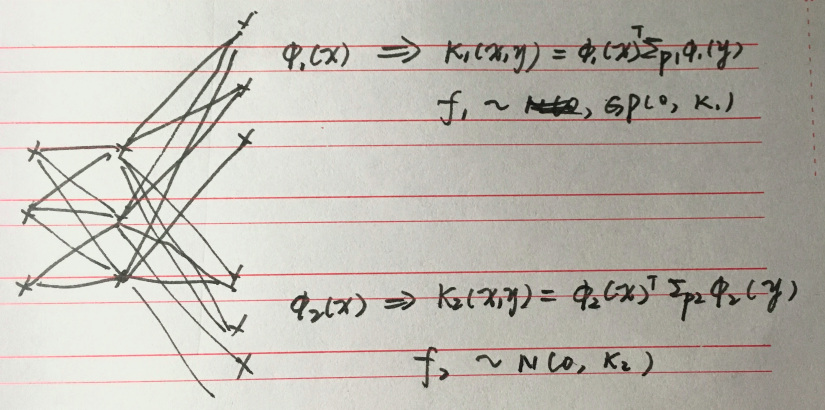
\includegraphics[width=\columnwidth]{./img/NN-MOGP.png}
    \caption{Architecture of the multi-output Gaussian process model.}
    \label{fig:MONNGP}
\end{figure}

We have shown that a GP can be constructed from a neural network with finite hidden units in the last layer. Now, we will show how to model the correlations between tasks and how to construct a multi-output Gaussian process model based on neural network.

Suppose we have $N$ observations $D_Q = \{X, Y | X \in R^{D \times N}, Y \in R^{N \times Q}\}$, we assume they are generated by $Q$ latent functions and polluted by noises with different noise level. Instead of building $Q$ independent models, we build a multi-output model that makes use of the correlations between the $Q$ tasks. Firstly, a neural network is used to define a \emph{shared feature map} $\phi_s : R^D \rightarrow R^{M_s}$. Then, for each task $i \in \{1,~\dots~,Q\}$, the shared feature $\phi_s(\bm{x})$ is followed by a \emph{task-specific} neural network that defines a feature map $\phi_i : R^{M_s} \rightarrow R^{M_i}$. We assume the $i$-th latent function $f_i(\bm{x})$ follows a GP distribution $f_i \sim \mathcal{GP}(0, k_i)$ defined as follows:

\begin{equation}
    \label{eq:mo_kernel}
    \left\{
    \begin{array}{lll}
        y_i                 &=&    f_i(\bm{x}) + \epsilon_i  \\
        f_i                 &\sim& \mathcal{GP}(0, k_i)      \\
        \epsilon_i          &\sim& N(0, \sigma_{n, i}^2)     \\
        k_i(\bm{x}, \bm{y}) &=&    \phi_i(\phi_s(\bm{x}))^T~\frac{\sigma_{p, i}^2}{M_i}~\phi_i(\phi_s(\bm{y}))
    \end{array}
    \right.
\end{equation}

As illustrated in \Fref{fig:MONNGP}, by defining GP with kernel function of \eqref{eq:mo_kernel}, we actually defined a neural network architecture with shared layers and task-specific layers, which is a common architecture used in multi-task deep learning \cite{ruder2017overview}. The correlations between tasks are naturally encoded by the shared layers, while the task-specific features are further learnt from the shared features.

With the model define in \eqref{eq:mo_kernel}, different tasks are \emph{conditionally independent} given the shared features, each specific task still sees a neural network with the same architecture plotted in \Fref{fig:NNGP}. The inferences of $\mu(\bm{x})$ and $\sigma^2(\bm{x})$ are exactly the same as \eqref{eq:DegeneratePred}, and no additional overhead will be introduced. As different tasks are conditionally independent, the log likelihood of the training data can be expressed as the sum of the log likelihood of each specific task
\begin{equation}
    \label{eq:mo_likelihood}
    \log p(Y | X, \bm{\Theta}) = \sum_{i=1}^Q \log p(\bm{y}_i | X, \bm{\theta}_i, \bm{\theta}_s),
\end{equation}
where $\bm{y}_i$ is the $i$-the column of $Y$, $\bm{\Theta}$ is the vector of all the parameters, including the shared parameters and the task-specific parameters. $\bm{\theta_i}$ is the vector of parameters for specific task $i$, including the weights of the $i$-th task-specific neural network, the weight prior factor $\sigma_{p, i}$ and the noise level $\sigma_{n, i}$ for the $i$-th task. $\bm{\theta}_s$ is a vector of the weights of the shared layers. The parameters $\bm{\Theta}$ are obtained by maximizing the likelihood function in \eqref{eq:mo_likelihood} with gradient back-propagation. The model averaging technique as described in subsection \ref{sec:deepensemble} is also employed in our model to improve the quality of uncertainty estimation. $K$ independent neural network models are trained with random initializations in our model. According to \eqref{eq:DegenerateGPloglikelihood} and \eqref{eq:mo_likelihood}, the time complexity of training for our model is $O(KN\sum_i^Q M_i^2)$.

\section{Experimental Results}\label{sec:report}

\subsection{ENB}\label{sec:enb}

\begin{itemize}
\item
  700 training
\item
  68 test
\item
  8 inputs
\item
  2 outputs
\end{itemize}

\begin{longtable}[]{@{}lll@{}}
\caption{SMSE of the ENB dataset (small is better)}\tabularnewline
\toprule
Algo & Output1 & Output 2\tabularnewline
\midrule
\endfirsthead
\toprule
Algo & Output1 & Output 2\tabularnewline
\midrule
\endhead
modsk: & 0.00155 \(\pm\) 0.000159 & 0.00753 \(\pm\)
0.00135\tabularnewline
igp: & 0.00188 \(\pm\) 2.29e-19 & 0.00911 \(\pm\)
1.83e-18\tabularnewline
cogp: & 0.00597 \(\pm\) 0.00088 & 0.0144 \(\pm\) 0.000831\tabularnewline
multigp: & 0.708 \(\pm\) 3.78e-05 & 1.21 \(\pm\) 4.1e-05\tabularnewline
npv: & 6.87 \(\pm\) 9.36e-16 & 8.63 \(\pm\) 1.87e-15\tabularnewline
mf: & 0.359 \(\pm\) 0.225 & 0.614 \(\pm\) 0.339\tabularnewline
\bottomrule
\end{longtable}

\begin{longtable}[]{@{}lll@{}}
\caption{NLL of the ENB dataset (small is better)}\tabularnewline
\toprule
Algo & Output1 & Output 2\tabularnewline
\midrule
\endfirsthead
\toprule
Algo & Output1 & Output 2\tabularnewline
\midrule
\endhead
modsk: & 0.332 \(\pm\) 0.0634 & 0.972 \(\pm\) 0.107\tabularnewline
igp: & 0.538 \(\pm\) 0 & 1.01 \(\pm\) 0\tabularnewline
cogp: & 1.34 \(\pm\) 0.159 & 2.08 \(\pm\) 0.212\tabularnewline
multigp: & 1.56 \(\pm\) 0.00363 & 1.66 \(\pm\) 0.00063\tabularnewline
npv: & NA & NA\tabularnewline
mf: & NA & NA\tabularnewline
\bottomrule
\end{longtable}

\subsection{SARCOS}\label{sec:sarcos}

\begin{itemize}
\item
  44484 training
\item
  4449 test
\item
  21 inputs
\item
  2 outputs
\item
  multigp: subset of data: use 2000 training set
\item
  GPRN-AVI: NIPS2017, black-box likelihood, M/N = 0.04
\item
  multigp gives zero prediction, underfitting
\end{itemize}

\begin{longtable}[]{@{}lll@{}}
\caption{SMSE of the SARCOS dataset (small is better)}\tabularnewline
\toprule
Algo & Output1 & Output 2\tabularnewline
\midrule
\endfirsthead
\toprule
Algo & Output1 & Output 2\tabularnewline
\midrule
\endhead
modsk: & 0.00156 \(\pm\) 3.46e-05 & 0.00307 \(\pm\)
5.64e-05\tabularnewline
igp: & 0.0045 \(\pm\) 0.000153 & 0.00787 \(\pm\) 0.000257\tabularnewline
cogp: & 0.00852 \(\pm\) 0.000241 & 0.0149 \(\pm\)
0.000433\tabularnewline
multigp: & 4.7 \(\pm\) 0.0245 & 3.39 \(\pm\) 0.0192\tabularnewline
npv: & Inf \(\pm\) NaN & Inf \(\pm\) NaN\tabularnewline
mf: & Inf \(\pm\) NaN & Inf \(\pm\) NaN\tabularnewline
\bottomrule
\end{longtable}

\begin{longtable}[]{@{}lll@{}}
\caption{NLL of the SARCOS dataset (small is better)}\tabularnewline
\toprule
Algo & Output1 & Output 2\tabularnewline
\midrule
\endfirsthead
\toprule
Algo & Output1 & Output 2\tabularnewline
\midrule
\endhead
modsk: & 0.804 \(\pm\) 0.0111 & -0.509 \(\pm\) 0.00813\tabularnewline
igp: & 1.06 \(\pm\) 0.00941 & -0.236 \(\pm\) 0.0124\tabularnewline
cogp: & 2.48 \(\pm\) 0.0577 & 2.4 \(\pm\) 0.097\tabularnewline
multigp: & 4.63 \(\pm\) 0.0128 & 2.87 \(\pm\) 0.011\tabularnewline
npv: & Inf \(\pm\) NaN & Inf \(\pm\) NaN\tabularnewline
mf: & Inf \(\pm\) NaN & Inf \(\pm\) NaN\tabularnewline
\bottomrule
\end{longtable}

\subsection{DAC14}\label{sec:dac14}

\begin{itemize}
\item
  2000 training
\item
  8000 test
\item
  10 inputs
\item
  15 outputs
\end{itemize}

\begin{longtable}[]{@{}llll@{}}
\caption{SMSE for DAC14 dataset}\tabularnewline
\toprule
Out & MOESK & IGP & COGP\tabularnewline
\midrule
\endfirsthead
\toprule
Out & MOESK & IGP & COGP\tabularnewline
\midrule
\endhead
O1 & 0.00064 \(\pm\) 3.5e-05 & 0.2 \(\pm\) 0.0019 & 0.19 \(\pm\)
0.0033\tabularnewline
O2 & 0.0006 \(\pm\) 3.9e-05 & 0.18 \(\pm\) 0.0061 & 0.15 \(\pm\)
0.0034\tabularnewline
O3 & 0.00054 \(\pm\) 4.2e-05 & 0.084 \(\pm\) 0.0034 & 0.084 \(\pm\)
0.0016\tabularnewline
O4 & 0.00023 \(\pm\) 1.7e-05 & 0.22 \(\pm\) 0.0037 & 0.053 \(\pm\)
0.0014\tabularnewline
O5 & 0.00028 \(\pm\) 2.1e-05 & 0.4 \(\pm\) 0.0053 & 0.087 \(\pm\)
0.0015\tabularnewline
O6 & 0.00022 \(\pm\) 1.4e-05 & 0.24 \(\pm\) 0.0024 & 0.049 \(\pm\)
0.00096\tabularnewline
O7 & 0.0013 \(\pm\) 9.6e-05 & 0.63 \(\pm\) 0.02 & 0.22 \(\pm\)
0.0031\tabularnewline
O8 & 0.0011 \(\pm\) 0.00014 & 0.45 \(\pm\) 0.013 & 0.15 \(\pm\)
0.0017\tabularnewline
O9 & 0.0011 \(\pm\) 0.00013 & 0.12 \(\pm\) 0.0021 & 0.073 \(\pm\)
0.0016\tabularnewline
O10 & 0.0011 \(\pm\) 9.8e-05 & 0.4 \(\pm\) 0.077 & 0.25 \(\pm\)
0.0036\tabularnewline
O11 & 0.001 \(\pm\) 0.00011 & 0.47 \(\pm\) 0.069 & 0.18 \(\pm\)
0.0038\tabularnewline
O12 & 0.00097 \(\pm\) 6.3e-05 & 0.39 \(\pm\) 0.087 & 0.1 \(\pm\)
0.0016\tabularnewline
O13 & 0.00032 \(\pm\) 2.3e-05 & 0.092 \(\pm\) 0.0038 & 0.092 \(\pm\)
0.00096\tabularnewline
O14 & 0.00036 \(\pm\) 2.9e-05 & 0.14 \(\pm\) 0.0052 & 0.11 \(\pm\)
0.0024\tabularnewline
O15 & 0.00027 \(\pm\) 1.4e-05 & 0.059 \(\pm\) 0.00043 & 0.059 \(\pm\)
0.00083\tabularnewline
\bottomrule
\end{longtable}

\begin{longtable}[]{@{}llll@{}}
\caption{LL for DAC14 dataset}\tabularnewline
\toprule
Out & MOESK & IGP & COGP\tabularnewline
\midrule
\endfirsthead
\toprule
Out & MOESK & IGP & COGP\tabularnewline
\midrule
\endhead
O1 & -2.3 \(\pm\) 0.033 & 0.43 \(\pm\) 0.0048 & 4.7 \(\pm\)
0.17\tabularnewline
O2 & -2.5 \(\pm\) 0.025 & 0.18 \(\pm\) 0.0079 & 3.3 \(\pm\)
0.25\tabularnewline
O3 & -2.4 \(\pm\) 0.026 & -0.1 \(\pm\) 0.01 & 3.2 \(\pm\)
0.15\tabularnewline
O4 & -3 \(\pm\) 0.038 & -1.1 \(\pm\) 0.018 & 2.1 \(\pm\)
0.14\tabularnewline
O5 & -3.1 \(\pm\) 0.037 & -1.1 \(\pm\) 0.035 & 2.1 \(\pm\)
0.14\tabularnewline
O6 & -3 \(\pm\) 0.03 & -0.95 \(\pm\) 0.011 & 1.8 \(\pm\)
0.21\tabularnewline
O7 & -2.2 \(\pm\) 0.042 & -0.74 \(\pm\) 0.047 & 5.7 \(\pm\)
0.4\tabularnewline
O8 & -2.4 \(\pm\) 0.055 & -1 \(\pm\) 0.041 & 4.8 \(\pm\)
0.36\tabularnewline
O9 & -2.2 \(\pm\) 0.036 & -1 \(\pm\) 0.024 & 2.5 \(\pm\)
0.18\tabularnewline
O10 & -2.1 \(\pm\) 0.052 & 0.32 \(\pm\) 0.045 & 5 \(\pm\)
0.4\tabularnewline
O11 & -2.2 \(\pm\) 0.067 & -0.031 \(\pm\) 0.033 & 4 \(\pm\)
0.13\tabularnewline
O12 & -2.1 \(\pm\) 0.025 & -0.27 \(\pm\) 0.018 & 3.7 \(\pm\)
0.24\tabularnewline
O13 & -2.7 \(\pm\) 0.032 & 0.049 \(\pm\) 0.0063 & 2.7 \(\pm\)
0.16\tabularnewline
O14 & -2.7 \(\pm\) 0.035 & -0.046 \(\pm\) 0.0055 & 2.4 \(\pm\)
0.24\tabularnewline
O15 & -2.7 \(\pm\) 0.023 & -0.2 \(\pm\) 0.0042 & 2.5 \(\pm\)
0.17\tabularnewline
\bottomrule
\end{longtable}


\section{Discussion}

Our model is effective, but it has several limitations, including the loss function, missing data...we plan to improve it in the future. 


% XXX:
% DNGO
% Deep-Kernel-Learning
% DNN-GP

\FloatBarrier

\bibliographystyle{unsrt}
\bibliography{ref.bib}

\end{document}
